\documentclass{article}
\usepackage[utf8]{inputenc}
\usepackage[margin=1in]{geometry}
\usepackage{crop,graphicx,amsmath,array,color,amssymb,flushend,stfloats,amsthm,chngpage,times,fancyhdr,lipsum,lastpage}
\usepackage{subcaption}
\numberwithin{equation}{section}
\usepackage[backend=biber,sorting=none]{biblatex}
\addbibresource{references.bib}

\renewcommand{\bottomfraction}{0.6}
\allowdisplaybreaks

%%%%%%%%%%%%   Header and Footer  %%%%%%%%%%%%%
\pagestyle{fancy}

\fancypagestyle{plain}{%
  \renewcommand{\headrulewidth}{0pt}%
  \fancyhf{}%
  \fancyfoot[R]{Page \bf\thepage\ \rm of \bf\pageref{LastPage}}%
}


%%%% Customise Titles and Headers: %%%%
\title{Project Proposal}
\author{Owen Rowell}
\date{\today}

\fancyhf{}
\fancyhead[L]{Owen Rowell}
\fancyhead[R]{1881130}
\fancyfoot[R]{Page \bf\thepage\ \rm of \bf\pageref{LastPage}}


\begin{document}

%%%%%%%%%%%% Make Title and Format Lines %%%%%%%%%%%%
\maketitle											%
\vspace{-112px}										%
\noindent\rule{\linewidth}{1pt} \par				%
\vspace{100px}										%
\vspace{-20px}										%
\noindent\rule{\linewidth}{1pt} \par				%
\vspace{10px}										%
%%%%%%%%%%%%%%%%%%% Insert Logos %%%%%%%%%%%%%%%%%%%%	
\vspace{-85px}										%
\noindent											%
\begin{minipage}{0.5\textwidth}\begin{flushleft}	%
\hspace{20px}										%

\includegraphics[scale = 0.06]{Resources/UoB}		%
\end{flushleft}\end{minipage}						%
\begin{minipage}{0.5\textwidth}\begin{flushright}	%

\includegraphics[scale = 0.06]{Resources/UoB}		%
\hspace*{20px}										%
\end{flushright}\end{minipage}						%
\vspace{20px}										%
%%%%%%%%%%%%%%%% Headers and Footers %%%%%%%%%%%%%%%%

\begin{abstract}
    This project aims to investigate the motion of vortices in high-$\kappa$ type-II superconductors. This report sets out the background theory required for this and discusses the method used to simulate such systems. Comparison of these simulations for the channel system is made to an analytical value of the critical shear showing the model to be running with an accuracy of $0.4\%$. The background theory of self-organised criticality and the avalanche system is then discussed prior to investigation next semester.
\end{abstract}
\tableofcontents

\newpage
\section{Introduction to Superconductivity}
\subsection{Key phenomena in superconductors}
Superconductivity was discovered by Heike Kamerlinah Onnes in 1911 when he was testing the effect of low temperature on the conduction of electricity in Mercury. He found that when cooled below a critical temperature of $T_c = 4.20K$, the resistance dropped below $10^{-5}\Omega$ - zero to within experimental errors \cite{VanDelft2010TheSuperconductivity}. This phenomenon of perfect conductivity can also be seen in many other metals below some characteristic temperature. In fact, currents are able to flow in a ring without any applied voltage with an experimental half-life of at least $10^5$ years \cite{Tinkham2004IntroductionSuperconductivity}.

Alongside perfect conduction, Meissner and Ochsenfeld also discovered in 1933 superconductors also exhibit perfect diamagnetism in their bulk \cite{Poole2014Superconductivity}. Whilst it could be expected that fields applied to a perfect conductor are excluded from it, they also found that any existing fields in the metal are expelled from the bulk as it is cooled below $T_c$ into a superconducting state. This phenomenon is called the Meissner effect and leads to all superconductors containing no magnetic flux except for an exponentially decaying `skin' at the boundary. This skin is characterised by the penetration depth of the superconductor, $\lambda$, which controls the decay of magnetic fields within the sample \cite{Tinkham2004IntroductionSuperconductivity}.

As well as superconductors only existing below a material dependent critical temperature $T_c$, the Meissner effect suggests that in order for the superconductor to be able to retain zero field in the bulk, the external field must also be suitably small. This leads to a critical field $H_c(T)$ above which the superconducting state is destroyed. This critical field is temperature dependent and has the approximate empirical form given by \cite{Tinkham2004IntroductionSuperconductivity}
\begin{equation}
    H_c(T) \approx H_c(0)[1 - (T/T_c)^2].
\end{equation}
It is important to note that the destruction of the superconducting state is unrelated to the source of such a critical field. This means that a field created by the current flowing through the superconductor itself can break superconduction, leading to the idea of a critical current density. For an infinitely long wire this has value \cite{Tinkham2004IntroductionSuperconductivity}
\begin{equation}
    J_c = \frac{H_c}{\lambda}.
\end{equation}
Above this, the field at the surface of the wire becomes greater than $H_c$ and the medium returns to its normal state.

The two properties of perfect conduction and diamagnetism were described mathematically in 1935 by F. and H. London through two equations now known as the London equations \cite{Poole2014Superconductivity}. These are
\begin{subequations}
\begin{align}
    \nabla \times \mathbf{j} &= -\frac{1}{\mu_0\lambda^2}\mathbf{B} \label{eqn:london1} \\
    \frac{\partial\mathbf{j}}{\partial t} &= \frac{1}{\mu_0\lambda^2}\mathbf{E} \label{eqn:london2},
\end{align}
\end{subequations}
where
\begin{equation}
    \frac{1}{\lambda^2} = \frac{\mu_0n_se^2}{m_e}. \label{eqn:pen_len}
\end{equation}
By substituting in Ampere's law, $\nabla \times \mathbf{B} = \mu_0 \mathbf{j}$, into equation~\ref{eqn:london1}, we get
\begin{align}
    \lambda^2\nabla^2\mathbf{B} &= \mathbf{B}\\
    \implies B &= B_0e^{-\frac{x}{\lambda}}
\end{align}
for a distance $x$ into the superconductor. This mathematically describes the Meissner effect of an exponentially decaying field within the superconductor, characterised by the penetration depth $\lambda$.

Equation~\ref{eqn:pen_len} relates $\lambda$ to $n_s(T)$, the superconducting electron density. This is the number of electrons per unit volume that are able to carry a supercurrent - lower than the normal electron density $n$. This number is temperature dependent and tends to zero at $T_c$ leading to a return to the normal state. Similarly, if we consider the boundary of a superconducting and normal metallic state, we could expect to see $n_s$ decay to zero across the boundary according to some characteristic length $\xi(T)$. This can be calculated from Ginzburg-Landau theory, in terms of a temperature dependent parameter $\alpha(T)$ related to the free energy \cite{Tinkham2004IntroductionSuperconductivity}
\begin{equation}
    \xi^2(T) = \frac{\hbar^2}{2m^*|\alpha(T)|}.
\end{equation}
This parameter is called the coherence length which along with the penetration depth $\lambda$ governs the behaviour of superconductors. Most important is the ratio between these \cite{Tinkham2004IntroductionSuperconductivity}
\begin{equation}
    \kappa = \frac{\lambda}{\xi}.
\end{equation}
This is called the Ginzburg-Landau parameter and is responsible for the separation of superconductors into two distinct types.

\subsection{Type II}
The superconductors discussed so far are more specifically known as type I superconductors and are categorised as those for which $\kappa < \frac{1}{\sqrt{2}}$. In 1957, Abrikosov discovered what are now referred to as type II superconductors \cite{Abrikosov1957TheAlloys}. For values of $\kappa > \frac{1}{\sqrt{2}}$, boundaries between normal and superconducting states become preferable to the free energy. This causes regions of the material to return to the normal state above some new critical field $H_{c1}$. These take the form of tubes of metallic state through the material which due to their normal state, now allow magnetic flux to enter the superconductor. As the field increases, more of these vortices form to further minimise the free energy through the creation of boundaries, until at some second critical field $H_{c2} = \sqrt{2}\kappa H_c$ the whole material has returned to a normal state.

Ginzburg-Landau theory requires that in order to retain single-valuedness of the order parameter, each vortex must carry an integer number of flux quanta
\begin{equation}
    \Phi_0 = \frac{h}{2e}.
\end{equation}
Since boundaries are energetically preferable, each vortex will carry as little flux as possible whilst all other flux forms new vortices. This means that each vortex carries exactly one quantum of flux $\Phi_0$ with larger fields causing more vortices within the medium \cite{Poole2014Superconductivity}. As with any magnetic field, the flux through each vortex induces a supercurrent in the superconducting medium surrounding it. Since such currents then interact with the field in other vortices, a repulsive force is created between the vortices. This repulsion causes the vortices to form a lattice, with this generally being triangular.

It is simplest to study the interaction of these vortices in the high-$\kappa$ limit. This is an acceptable limit in superconductors such as copper oxides which can have $\kappa \approx 100$ \cite{Poole2014Superconductivity}. Here the fields from vortices do not overlap and can so can be approximated as a Dirac delta function of flux at the location of the vortex. Adding this term to the first London equation (equation~\ref{eqn:london1}) and solving gives the field due to one vortex to be \cite{Poole2014Superconductivity}
\begin{equation}
    B(r) = \frac{\Phi_0}{2\pi\lambda^2}K_0\left(\frac{r}{\lambda}\right),
\end{equation}
where $K_0(z)$ is the modified Bessel function of the first kind with order zero. The current induced by this vortex is then found using Maxwell's equation
\begin{align}
    \mathbf{J} &= \frac{1}{\mu_0}\nabla\times\mathbf{B} \nonumber \\
    \implies J(r) &= \frac{\Phi_0}{2\pi\mu_0\lambda^3}K_1\left(\frac{r}{\lambda}\right).
\end{align}
This causes a force to be exerted on the other vortices due to the Lorentz interaction between the current and field within the vortex. This gives a force on vortex 2 due to vortex 1 as
\begin{equation}
    \mathbf{F}_{21} = f_0K_1\left(\frac{|\mathbf{r}_{12}|}{\lambda}\mathbf{\hat{r}_{12}}\right), \label{eqn:vortex_force}
\end{equation}
where $\mathbf{\hat{r}_{12}}$ is the vector from vortex 1 to vortex 2 and $f_0 = \frac{\Phi_0^2}{2\pi\mu_0\lambda^3}$. It is this interaction and the interaction of vortices with external forces, that will drive the investigations within this project.

\section{The vortex channel system}
\subsection{The Lorentz force}
The interaction between vortices due to the Lorentz force has already been discussed in the previous section. However, this can also create a force due to an applied current flowing through the superconducting bulk. As we have
\begin{equation}
    \mathbf{F}_I = \mathbf{J} \times \mathbf{\Phi_0}, \label{eqn:lorentz_f}
\end{equation}
acting on any given vortex, this is independent of the position or motion of all other vortices so can be treated as a constant force $\mathbf{F}_I$ acting on every vortex. The cross product in equation~\ref{eqn:lorentz_f} requires that this force is perpendicular to the flux so will act in the same plane as all other vortex motion due to the vortex-vortex interaction.

This force leads to a flow of vortices through the superconductor perpendicular to the applied current. Such movement induces an electric field that resists the applied voltage, hence breaking perfect conductivity \cite{Tinkham2004IntroductionSuperconductivity}. However, flux flow can be prevented by pinning the vortices in place so that the Lorentz force cannot move them, thus allowing the resistance to stay at zero. Pinning is caused by defects within the superconductor - either naturally occurring or intentionally introduced through doping. As long as the current is low enough that the Lorentz force is below the pinning force, these vortices will remain stationary and a supercurrent is able to flow in the superconducting state around them \cite{Poole2014Superconductivity}.

\subsection{The channel system}
We have now laid out the basis on which the flux vortices move and interact, from this we can create a channel system in which to investigate their behaviour.
First suggested in 1988 by Pruymboom et al., the channel is made by pinning vortices in the superconductor in their ground state lattice, except for a channel of vortices that are left free to flow. Experimentally, Pruymboom achieved this by placing a layer of NbN, which exhibits strong pinning, on top of a layer of amorphous Nb$_3$Ge, which has weak pinning. Due to the thinness of the layers, the vortices pinned in the NbN layer continue through the Nb$_3$Ge with little deviation, hence also effectively pinning them within the Nb$_3$Ge. By cutting channels in the NbN layer, the strong pinning is removed leaving a channel of free flowing flux vortices \cite{Pruymboom1988Flux-lineFilms}.

Figure~\ref{fig:channel_system} shows a section of this system in the simplest case of a two lattice spacings wide channel containing one line of free vortices.
\begin{figure}[htb]
    \centering
    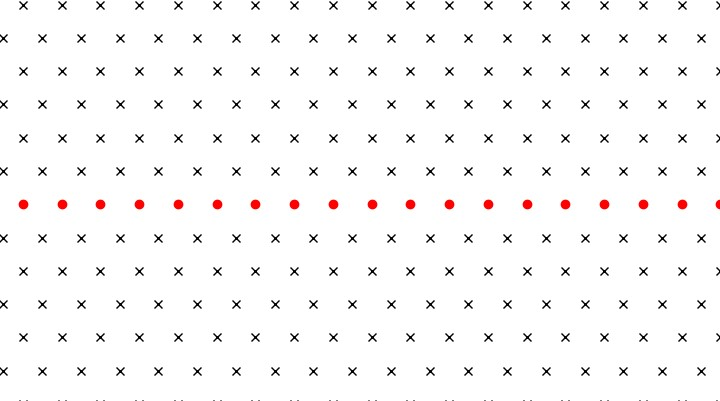
\includegraphics[width=0.8\linewidth]{results/Figures/channel_drawing - cropped.jpg}
    \caption{The channel system with width 1 - crosses represent pinned vortices and red dots represent vortices free to flow along the channel.}
    \label{fig:channel_system}
\end{figure}
In reality, this is a 3d system with the vortices coming out of the page through the block of superconductor. However, as long as the weakly pinning layer is thin, we only need to consider a single 2d plane as the position of the vortices will not vary much through the system \cite{Gartlan2020NovelFibres}.
 
\subsection{Critical shear} \label{sec:critical_shear}
An important quantity of the channel system is the critical shear - the minimum force from the applied current required for the vortices to flow along the channel. For forces below this, the vortices will remain in the wells of the washboard potential created by the pinned vortices as shown in figure~\ref{fig:washboard_f0}. The addition of the constant Lorentz force is a linear increase to the potential causing these wells to `tip', thus reducing their size. Eventually, for some $\mathbf{F}=\mathbf{F}_c$, the potential wells cease to be wells at all and the vortices will begin to flow along the channel as seen in figure~\ref{fig:washboard_fc} \cite{Gartlan2020NovelFibres, Watkins2016DensitySuperconductors}. We can also expect that for $\mathbf{F}\gg\mathbf{F}_c$, the original washboard will be negligible compared to the potential due to $\mathbf{F}$ and the vortices will flow as if only driven by the constant Lorentz force.
\begin{figure}[htb]
\centering
\begin{subfigure}[t]{.33\textwidth}
  \centering
  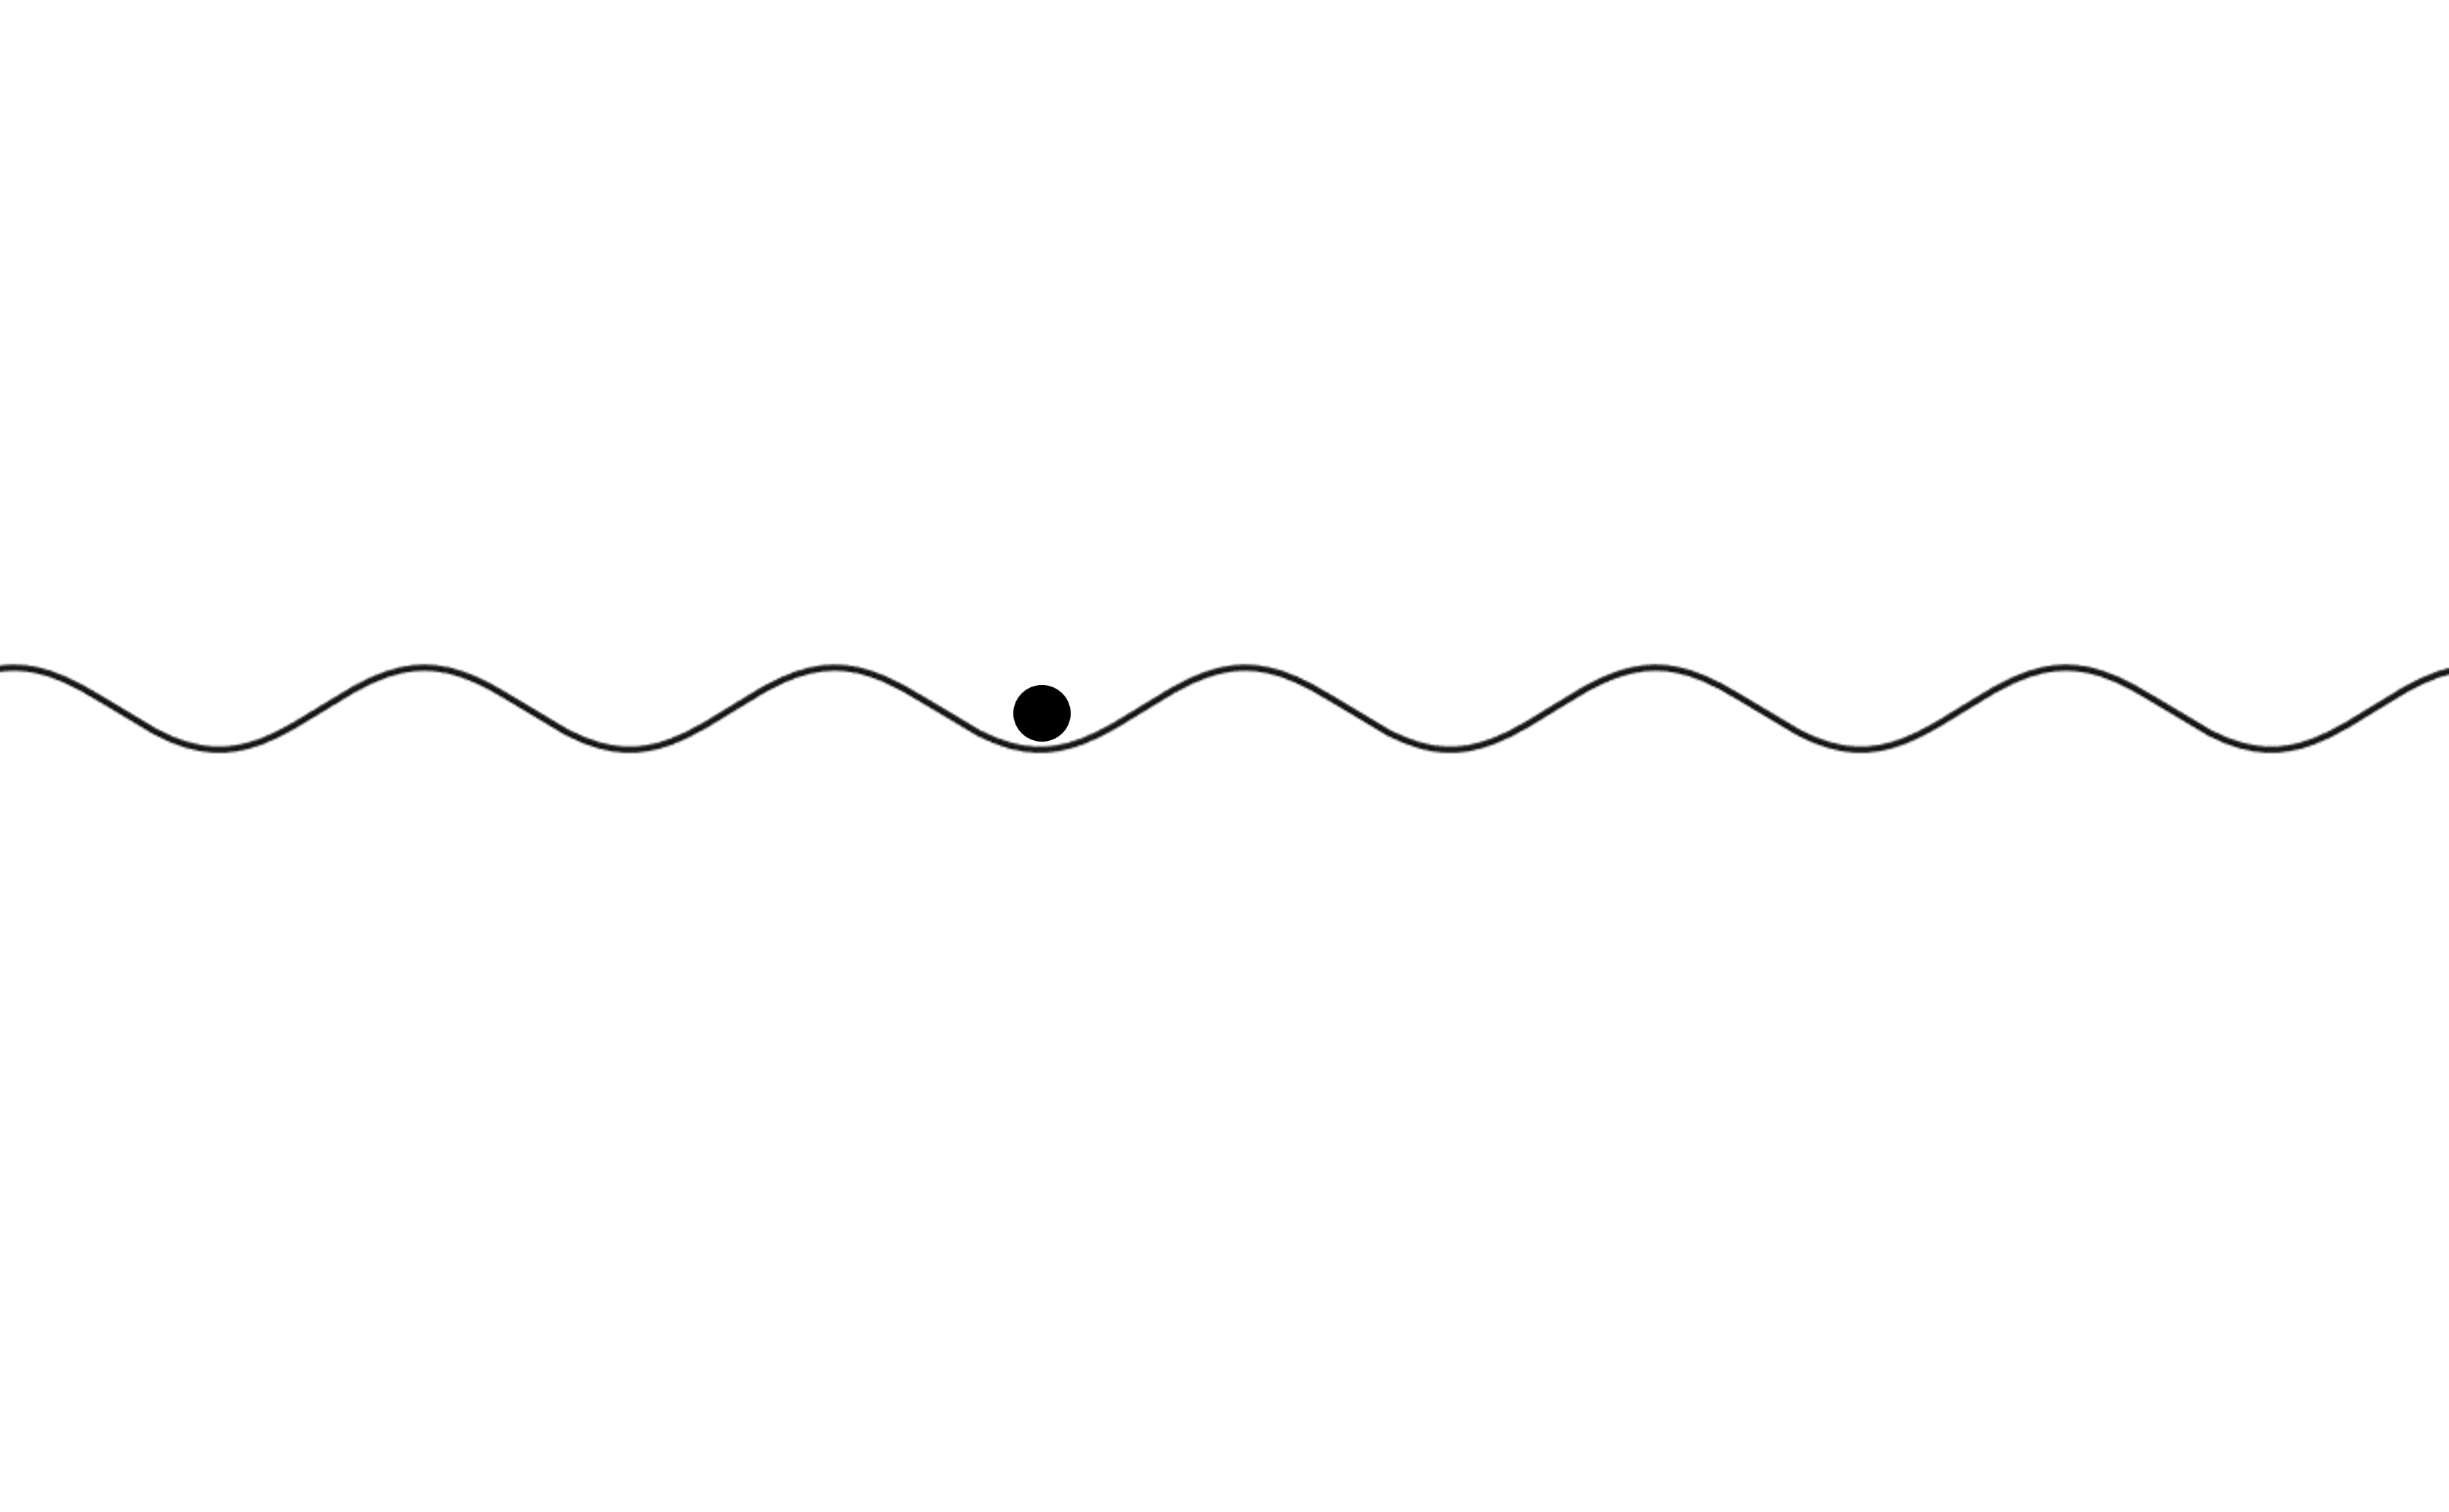
\includegraphics[width=.9\linewidth]{results/Figures/washboard-f0.png}
  \caption{$\mathbf{F}=0$}
  \label{fig:washboard_f0}
\end{subfigure}
\hfill
\begin{subfigure}[t]{.33\textwidth}
  \centering
  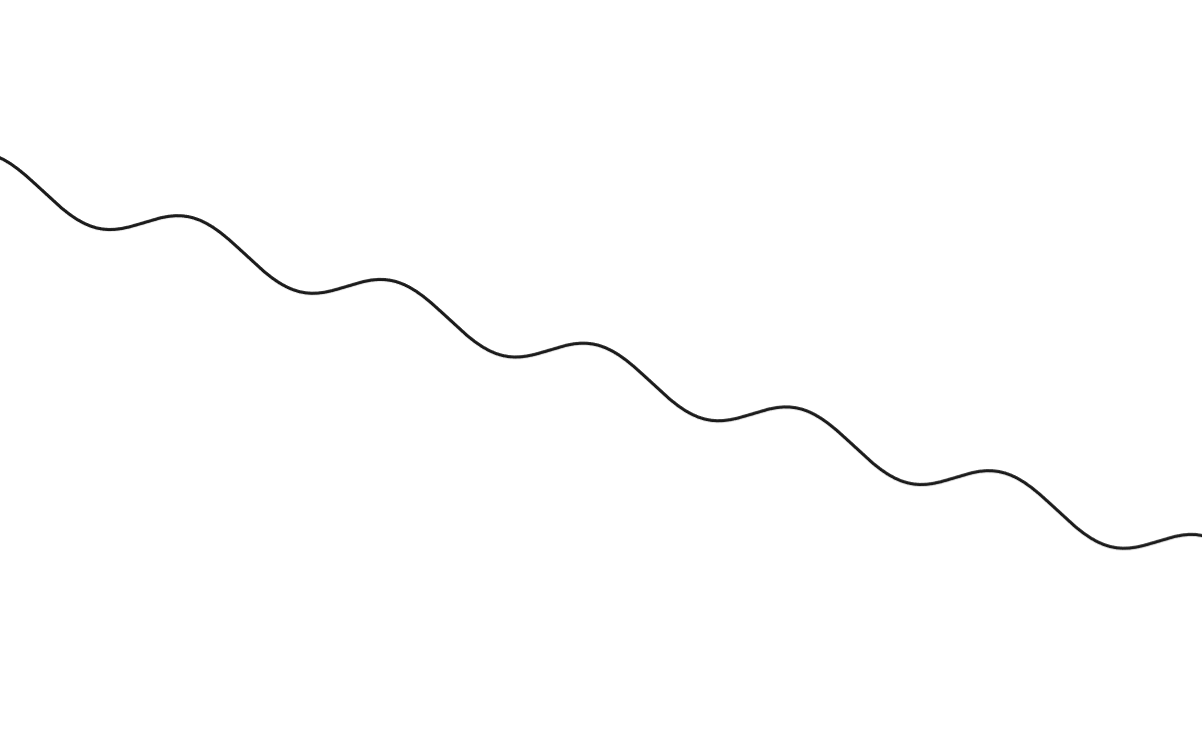
\includegraphics[width=.9\linewidth]{results/Figures/washboard-f.png}
  \caption{$0<\mathbf{F}<\mathbf{F}_c$}
  \label{fig:washboard_f}
\end{subfigure}
\hfill
\begin{subfigure}[t]{.33\textwidth}
  \centering
  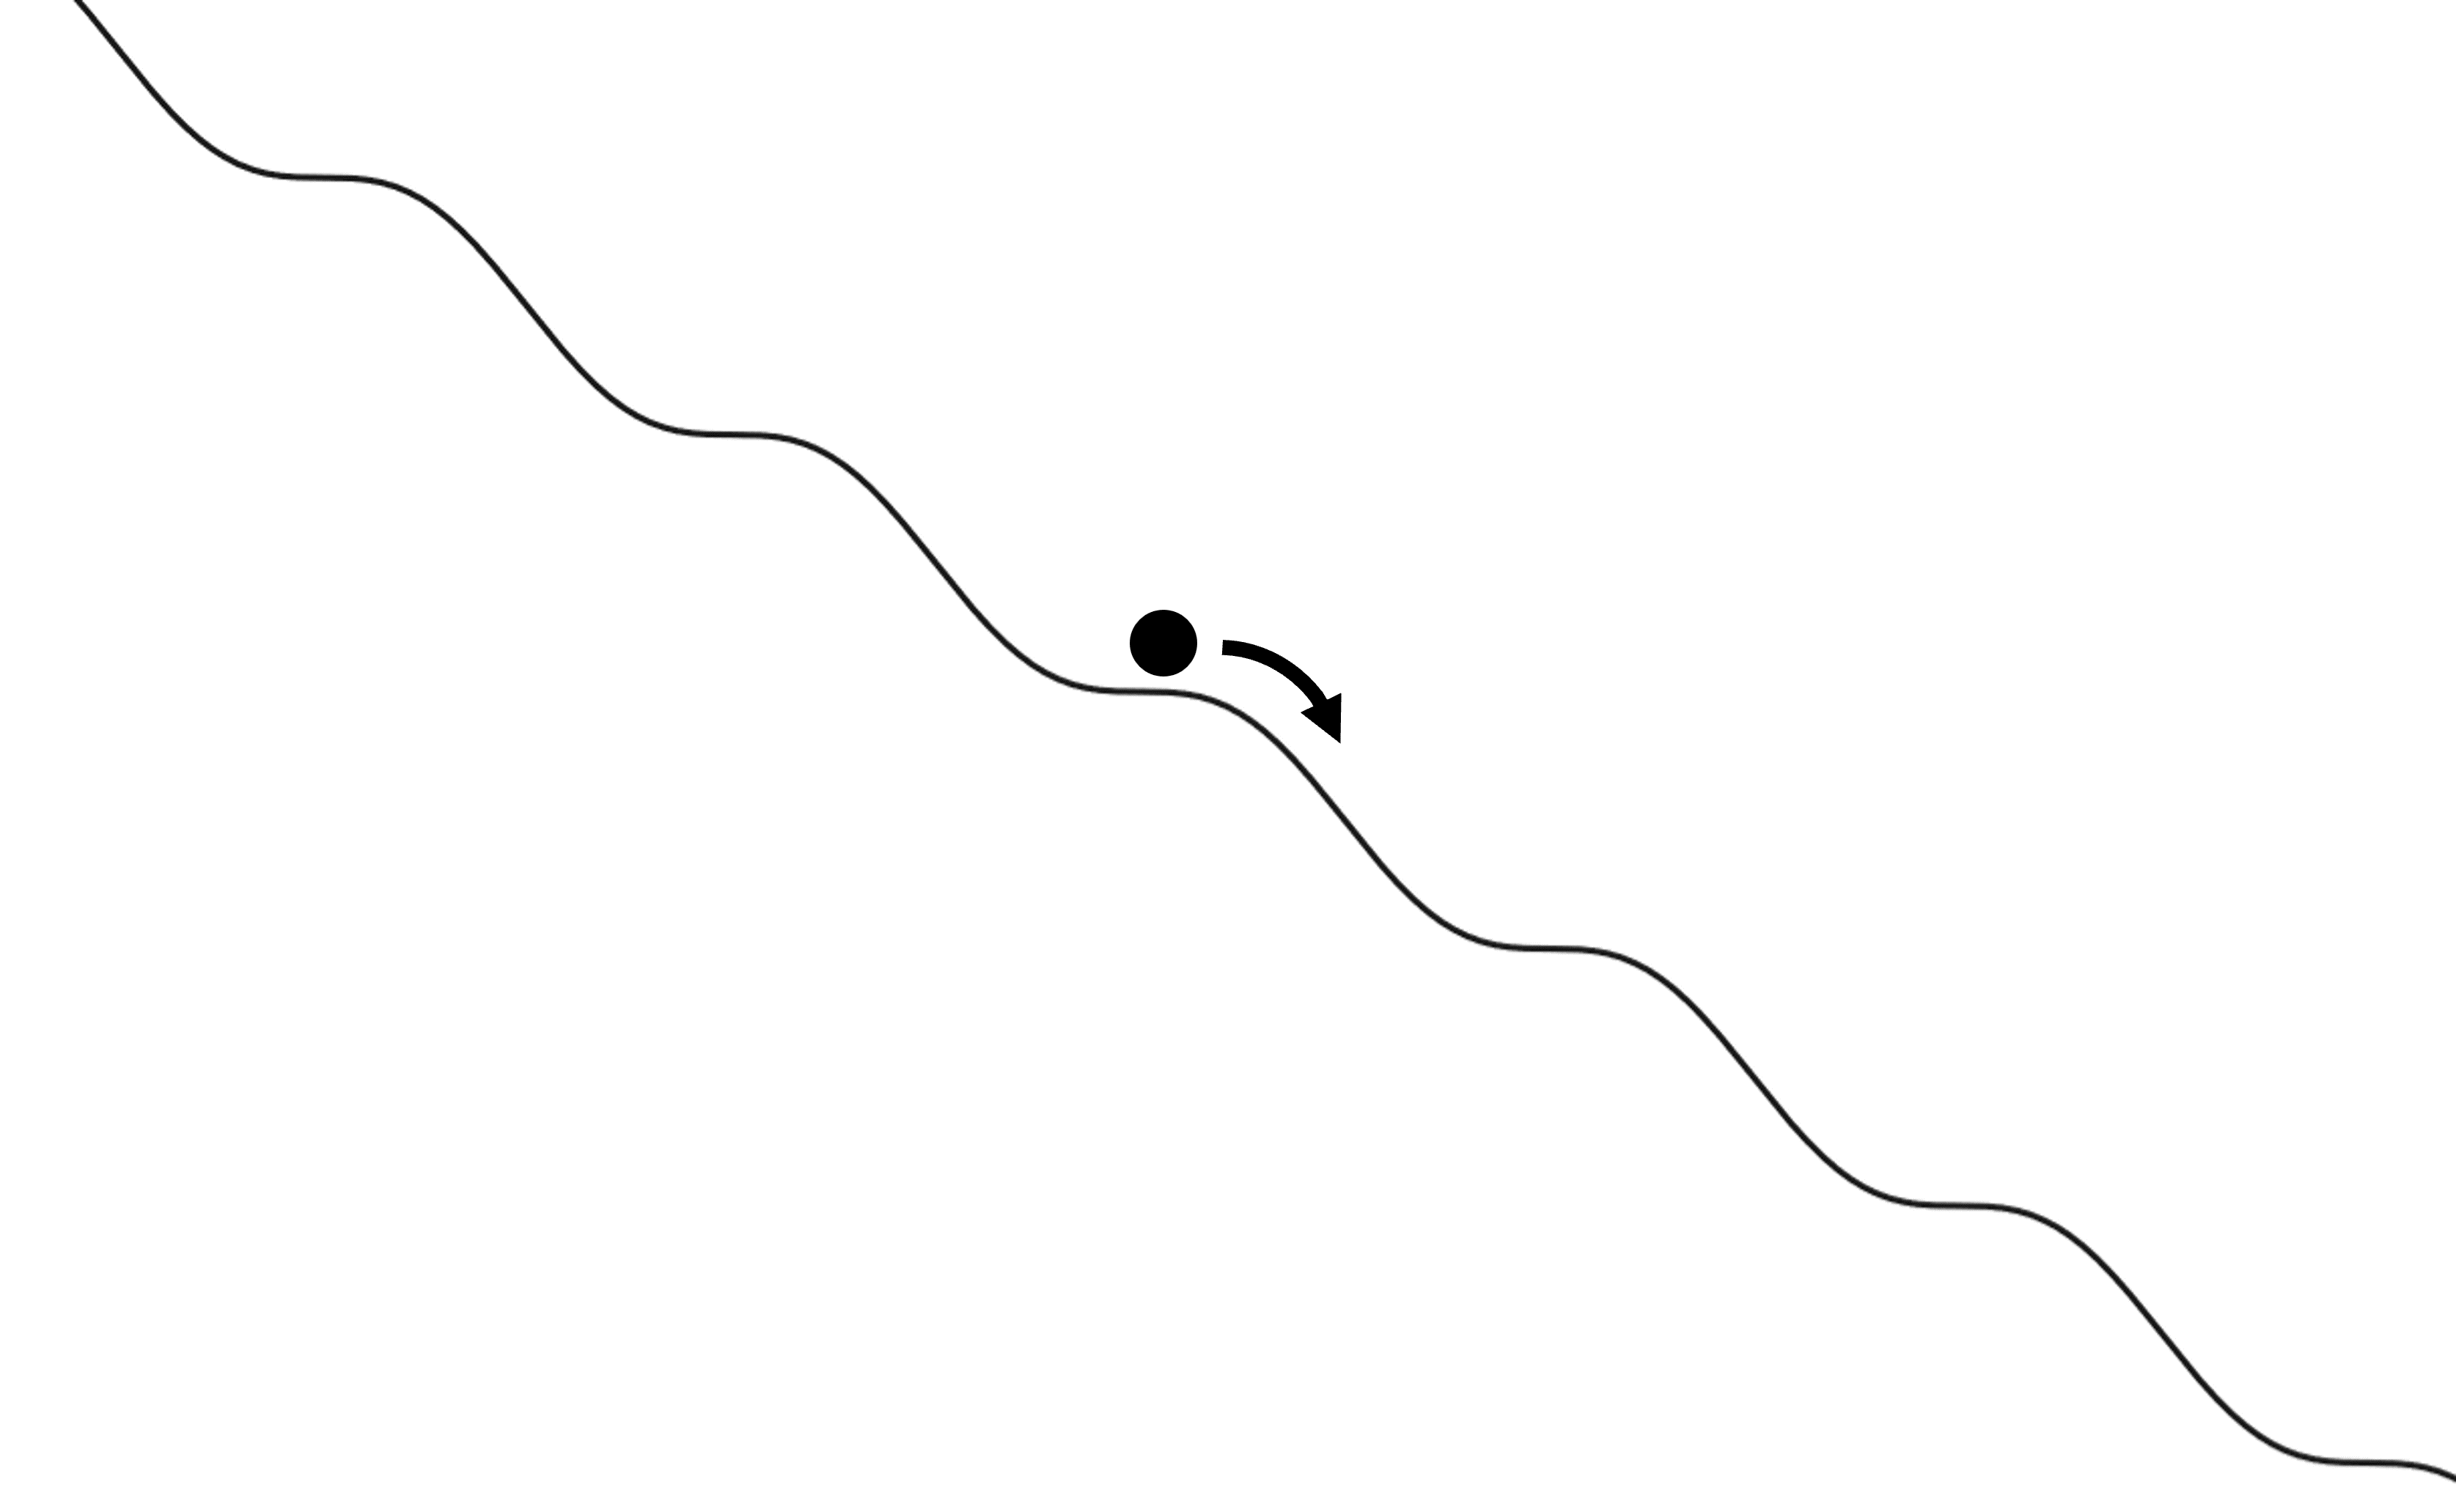
\includegraphics[width=.9\linewidth]{results/Figures/washboard-fc.png}
  \caption{$\mathbf{F}=\mathbf{F}_c$}
  \label{fig:washboard_fc}
\end{subfigure}
\caption{Washboard model of the potential for differing applied forces up to the critical shear.}
\label{fig:washboard}
\end{figure}

This quantity is a useful one to consider due to its ease of measurability, both experimentally and numerically as will be seen in section~\ref{sec:comp_crit_chear}. A range of currents can be applied to the system and the long-term motion of the vortices (if any) measured to find a cutoff point, $\mathbf{F}_c$, followed by a tend towards an asymptote $\mathbf{F} \propto \mathbf{v}$ assuming the existence of a terminal velocity.

\section{Simulation method}
Investigation of the channel system is done by simulating it through the use of molecular dynamics. This is done by integrating the equations of motion for each vortex using python with the numpy package. The Bessel function $K_1$ was provided through the scipy special functions library.
\subsection{Molecular dynamics}
In the case of large-$\kappa$, each vortex can be considered as a particle and we can use the Langevin equation, which in the case of zero temperature is given by
\begin{equation}
    m\ddot{\mathbf{x}} = \mathbf{F} - \eta\dot{\mathbf{x}}. \label{eqn:langevin}
\end{equation}
Here $\eta$ is the viscous drag on a vortex due to dissipative forces such as current flowing through the cores of the vortices which are in a non-superconducting state \cite{Bardeen1965TheorySuperconductors, Watkins2016DensitySuperconductors}. This applies to each free vortex in the system leading to a system of $2N$ coupled differential equations in the case where we take the vortices to be straight throughout the superconductor.

We first assume that the effect of this $\eta$ is much greater than that of the inertial term $m\ddot{\mathbf{x}}$, such that we can take $m=0$ and simplify equation~\ref{eqn:langevin} to
\begin{equation}
    \dot{\mathbf{x}} = \frac{1}{\eta}\mathbf{F}. \label{eqn:langevin_ovdamp}
\end{equation}
This is commonly called the overdamped Langevin equation and effectively assumes the particles instantly reach terminal velocity \cite{Poole2014Superconductivity}.
Integration of this equation is done using the Euler method to give the iterative equation
\begin{equation}
    \mathbf{x}_{n+1} = \mathbf{x}_n + \frac{\Delta t}{\eta}\mathbf{F}_n,
\end{equation}
where $\Delta t$ is some small time step at which forces are calculated and applied to the vortices.

The total force $\mathbf{F}$ in equation~\ref{eqn:langevin_ovdamp}, can be split into three contributing forces
\begin{equation}
    \mathbf{F} = \mathbf{F}_{vv} + \mathbf{F}_P + \mathbf{F}_I
\end{equation}
where:
\begin{itemize}
    \item $\mathbf{F}_{vv}$ is the force due to the vortex-vortex interaction. This is a sum of each individual force between the vortex being considered and every other vortex in the system as given by equation~\ref{eqn:vortex_force}.
    \item $\mathbf{F}_P$ is the force due to the pinned vortex lattice. Most simplistically, this force is done by the same calculation as for $\mathbf{F}_{vv}$, however due to the large number of vortex interactions this requires, a more efficient, analytical form can be used instead which is discussed later in section~\ref{sec:analytic_chan}.
    \item $\mathbf{F}_I$ is the Lorentz force due to the applied current. While this can be calculated using equation~\ref{eqn:lorentz_f}, it does not vary between vortices or over time, so a resulting constant force is just applied to each vortex.
\end{itemize}

\subsection{Optimisations}
Whilst physically, the channel system is very long and so contains many vortices, this is infeasible to simulate numerically. Instead, periodic boundary conditions are used at either end of the channel by wrapping any particles that flow off the end to the other side. In order to reduce end effects this would lead to, multiple images of the system are produced beyond the periodic boundaries. A force is then applied to each real vortex from the images as well as other real vortices.

The calculation of $\mathbf{F}_{vv}$ (and also $\mathbf{F}_P$ when done vortex by vortex) involves $N^2$ individual calculations of the repulsive force. These each involve calculating the value of the Bessel function $K_1$ which is very computationally expensive. To reduce this, a cutoff is used, beyond which it is assumed that any interactions are negligible and so the force taken to be zero. This means that the number of calls to the Bessel function is now $\sim N$ allowing a larger number of vortices to be simulated. However, since the number of vortices that a given vortex interacts with will grow as $r^2$, a cutoff of 9 lattice spacings was used to ensure that the next shell of discounted vortices is negligible, even if individual vortices closer than this exert very small forces.

To improve precision as well as making the results easier to read, constants are chosen such that the simulation generally works on order $1$. To do this we choose $\lambda = \eta = f_0 = a_x = 1$ which also gives $a_y = \frac{\sqrt{3}}{2}$.

\section{Simulation validation}
It is important to ensure that the simulation that has been written is behaving correctly. This can be done through a few tests that have known results and comparing these to those produced by the code.
\subsection{Ground state}
The first and most simple of these is the production of the ground state. Vortices placed in a triangular lattice with spacing $a_x=1$, $a_y=\frac{\sqrt{3}}{2}$ should remain in this state. Similarly, vortices placed in random locations should also arrange themselves into a triangular lattice.

This is done first with only four real vortices placed at $(0, 0)$, $(1, 0)$, $(\frac{1}{2}, \frac{\sqrt{3}}{2})$ and $(\frac{3}{2}, \frac{\sqrt{3}}{2})$ using various numbers of images in each direction. Note that if imaging is done 6 times each way, then a total of $13^2-1=168$ image grids are created. Table~\ref{tab:dist_from_images} shows the effect of the number of images on how closely to the ground state the simulation remained at.
\begin{table}[htb]
    \centering
    \begin{tabular}{c|c}
        Images used & Average distance moved from ground state \\
        \hline
        1 & $1.12\times 10^{-2}$ \\
        2 & $1.59\times 10^{-3}$ \\
        4 & $3.04\times 10^{-5}$ \\
        6 & $5.63\times 10^{-7}$ \\
        8 & $1.03\times 10^{-8}$ \\
        10 & $1.90\times 10^{-10}$ \\
    \end{tabular}
    \caption{Average distance away from the ground state travelled by vortices for differing numbers of image vortices in each direction.}
    \label{tab:dist_from_images}
\end{table}
From this, we see that the simulation does in fact remain in the ground state, provided enough images are used. Fewer images reduce accuracy as without the full repulsion of a surrounding ground state lattice, the repulsion between the four real vortices will cause them to spread out slightly more than the ground state.
\begin{figure}[htb]
\centering
\begin{subfigure}[t]{.49\textwidth}
    \centering
    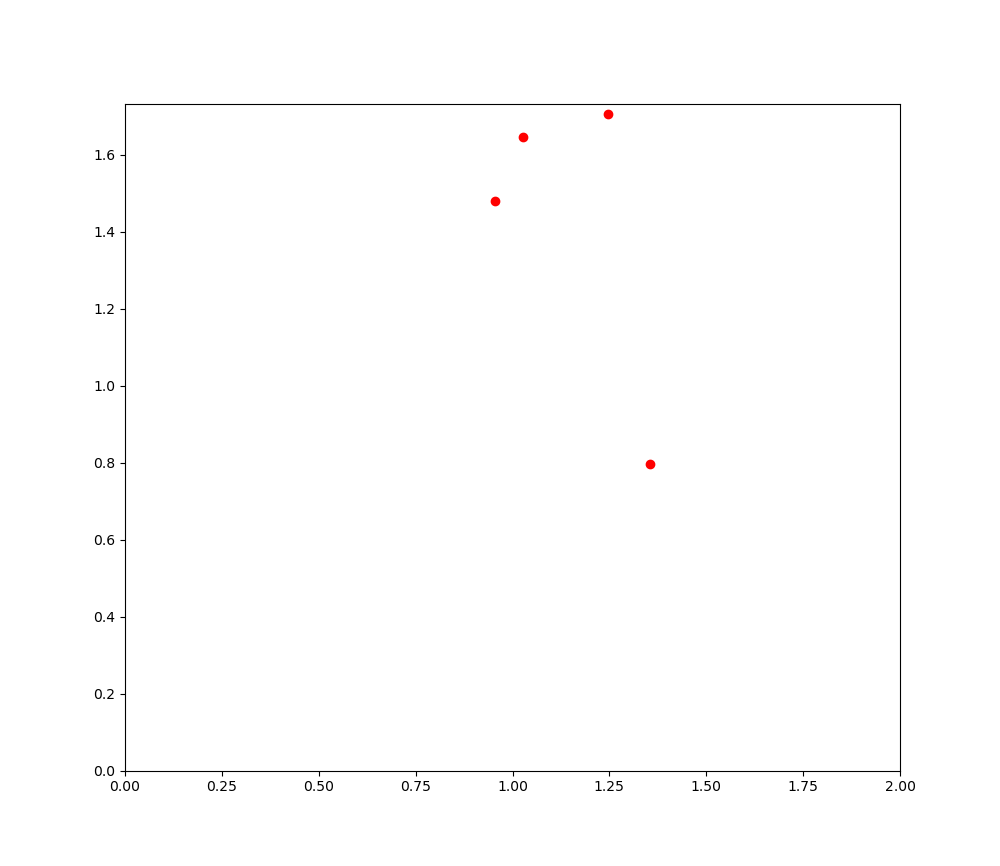
\includegraphics[width=.9\linewidth]{results/gifs/Basic_tests/ground_state_rand_000.png}
    \caption{Initial random state}
    \label{fig:ground_rand_000}
\end{subfigure}
\hfill
\begin{subfigure}[t]{.49\textwidth}
    \centering
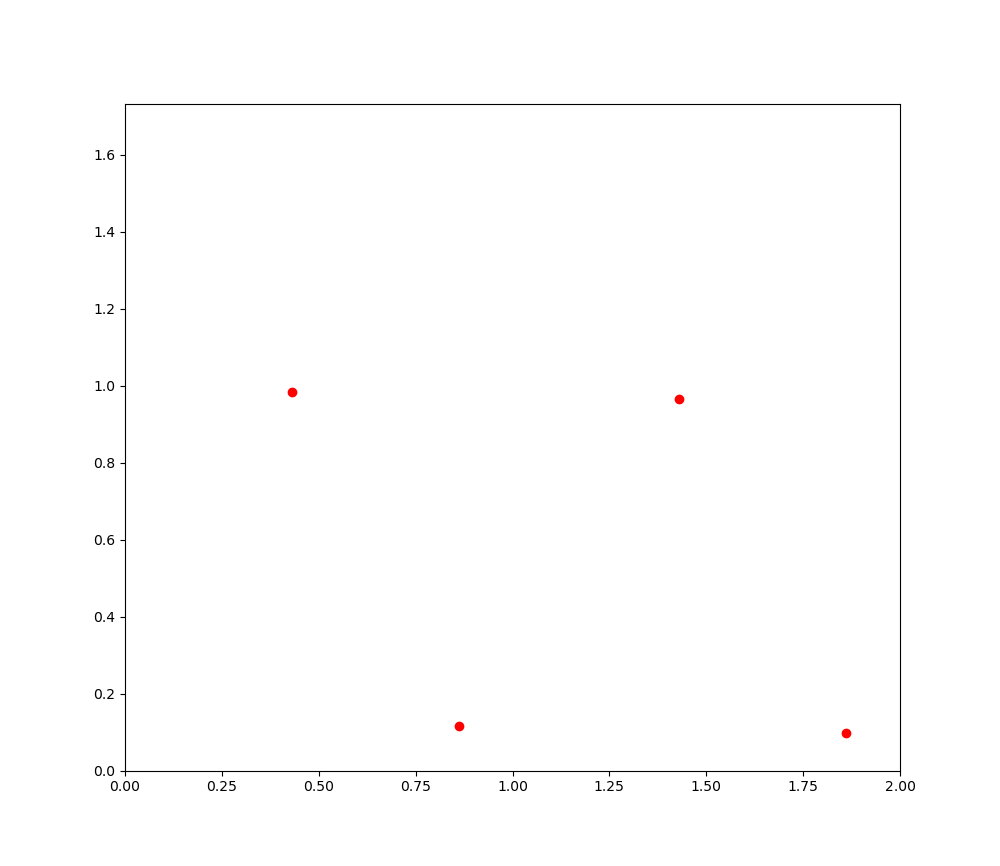
\includegraphics[width=.9\linewidth]{results/gifs/Basic_tests/ground_state_rand_749.png}
    \caption{State after 15 seconds}
    \label{fig:ground_rand_749}
\end{subfigure}
\caption{Simulation of four randomly placed vortices finding the ground state.}
\label{fig:ground_rand}
\end{figure}

Next, four vortices were initially placed in random positions and the simulation run to check that they would find the ground state. The positions of these initially and after 15 seconds can be seen in figure~\ref{fig:ground_rand} which, as expected, form a triangular lattice.

\subsection{Critical shear of the channel system} \label{sec:comp_crit_chear}
Given the success of these tests, we now look to simulating the channel system by including pinned vortices. As discussed in section~\ref{sec:critical_shear}, a good test to validate this system is the value for the critical shear that it produces. However, we first need a true value that we can compare to. This is done by replacing the lattice of vortices each exerting a force given by equation~\ref{eqn:vortex_force}, with a single force from the channel.

\subsubsection{Analytical form of the channel lattice} \label{sec:analytic_chan}
We start by using equation~\ref{eqn:vortex_force} to get the potential due to a line of pinned vortices along the x-axis of separation $a_x$ as \cite{Watkins2016DensitySuperconductors}
\begin{equation}
    V_L(x, y) = \frac{f_0}{\lambda}\sum_{n=-\infty}^\infty K_0 \left( \frac{\sqrt{(x + na_x)^2 + y^2}}{\lambda} \right).
\end{equation}
Writing the modified Bessel function using the form found in \cite{I.S.Gradshteyn2015TableProducts}
\begin{equation}
    K_0(z) = \frac{1}{2}\int_0^\infty \frac{\mathrm{d}t}{t}e^{-t-\frac{z^2}{4t}}
\end{equation}
allows the Fourier transform of the potential to be written as (neglecting the proportionality constant)
\begin{align*}
    \tilde{V}_L(k_x, k_y) &= \frac{1}{2}\sum_{n=-\infty}^\infty \int_{-\infty}^\infty\frac{\mathrm{d}x}{\sqrt{2\pi}}e^{ik_xx} \int_{-\infty}^\infty\frac{\mathrm{d}y}{\sqrt{2\pi}}e^{ik_y} \int_0^\infty\frac{\mathrm{d}t}{t}e^{-t-\frac{(x+na_x)^2 + y^2}{4\lambda^2t}} \\
    &= \frac{1}{2}\sum_{n=-\infty}^\infty \frac{\mathrm{d}t}{t}e^{-t} \int_{-\infty}^\infty\frac{\mathrm{d}x}{\sqrt{2\pi}}e^{-\frac{(x+na_x)^2}{4\lambda^2t}+ik_xx}
    \int_{-\infty}^\infty\frac{\mathrm{d}y}{\sqrt{2\pi}}e^{-\frac{y^2}{4\lambda^2t}+ik_yy}.
\end{align*}
Taking $x \rightarrow x - na_x$ and using the known result for the Gaussian integral
\begin{equation}
    \int_{-\infty}^\infty\frac{\mathrm{d}z}{\sqrt{2\pi}}e^{-\frac{z^2}{a}+bz} = \sqrt{\frac{a}{2}}e^{\frac{ab^2}{4}}
\end{equation}
gives
\begin{align*}
    \tilde{V}_L(k_x, k_y) &= \frac{1}{2}\sum_{n=-\infty}^\infty e^{-ina_xk_x} \int_0^\infty\frac{\mathrm{d}t}{t}e^{-t} \sqrt{\frac{4\lambda^2t}{2}}e^{\frac{4\lambda^2t(ik_x)^2}{4}} \sqrt{\frac{4\lambda^2t}{2}}e^{\frac{4\lambda^2t(ikyx)^2}{4}} \\
    &= \lambda^2\sum_{n=-\infty}^\infty e^{-ina_xk_x} \int_0^\infty\mathrm{d}te^{-t}e^{-\lambda^2k_x^2t}e^{-\lambda^2k_y^2t} \\
    &= \lambda^2\sum_{n=-\infty}^\infty e^{-ina_xk_x} \left[\frac{-1}{1+\lambda^2k_x^2+\lambda^2k_y^2} e^{-\left(1+\lambda^2k_x^2+\lambda^2k_y^2\right)t}\right]_0^\infty\ \\
    &= \sum_{n=-\infty}^\infty \frac{e^{-ina_xk_x}}{\frac{1}{\lambda^2}+k_x^2+k_y^2}.
\end{align*}
This is then Fourier transformed back using the formula for the Dirac comb
\begin{equation}
    \sum_{n=-\infty}^\infty\delta(k-Tn) = \frac{1}{T}\sum_{n=-\infty}^\infty e^{\frac{2\pi ikn}{T}},
\end{equation}
which gives
\begin{align*}
    V_L(x, y) &= \int_{-\infty}^\infty\frac{\mathrm{d}k_x}{\sqrt{2\pi}}e^{-ik_xx} \left(\sum_{n=-\infty}^\infty e^{-ina_xk_x}\right) \int_{-\infty}^\infty\frac{\mathrm{d}k_y}{\sqrt{2\pi}} \frac{e^{-ik_yy}}{\frac{1}{\lambda^2}+k_x^2+k_y^2} \\
    &= \int_{-\infty}^\infty\frac{\mathrm{d}k_x}{\sqrt{2\pi}}e^{-ik_xx} \left(\frac{2\pi}{a_x}\right)\sum_{n=-\infty}^\infty
    \delta\left(k_x - \frac{2\pi n}{a_x}\right) \int_{-\infty}^\infty\frac{\mathrm{d}k_y}{\sqrt{2\pi}} \frac{e^{-ik_yy}}{\frac{1}{\lambda^2}+k_x^2+k_y^2} \\
     &= \sum_{n=-\infty}^\infty e^{-\frac{2\pi ixn}{a_x}}\frac{1}{a_x} \int_{-\infty}^\infty\frac{e^{-ik_yy}} {\frac{1}{\lambda^2}+\left(\frac{2\pi n}{a_x}\right)^2+k_y^2}\mathrm{d}k_y.
\end{align*}
Letting $Q_n^2 = \frac{1}{\lambda^2} + \left(\frac{2\pi n}{a_x}\right)^2$ and doing the remaining integral finally gives
\begin{align}
    V_L(x, y) &= \frac{1}{a_x}\sum_{n=-\infty}^\infty e^{-\frac{2\pi in}{a_x}x} \int_{-\infty}^\infty\frac{e^{-ik_yy}} {Q_n^2+k_y^2}\mathrm{d}k_y \nonumber \\
    &= \frac{1}{a_x}\sum_{n=-\infty}^\infty e^{-\frac{2\pi in}{a_x}x}\cdot \frac{\pi}{Q_n}e^{-|y|Q_n} \nonumber \\
    &= \frac{\pi}{a_x}\sum_{n=-\infty}^\infty \frac{e^{-\frac{2\pi in}{a_x}x-Q_n|y|}}{Q_n}.
\end{align}
A semi-infinite sum over this line of vortices is then done to produce a triangular Abrikosov lattice that can form each side of the channel. This is done by increasing both the $x$ and $y$ offset of $V_L$ with each line
\begin{align*}
    V_A(x, y) &= \sum_{m=0}^\infty V_L\left(x+\frac{ma_x}{2},y+ma_y\right) \\
    &= \frac{\pi}{a_x}\sum_{n=-\infty}^\infty\frac{1}{Q_n}\sum_{m=0}^\infty
    e^{-i\frac{2\pi n}{a_x}x-Q_n|y|}e^{-mn\pi i-Q_nma_y} \\
    &= \frac{\pi}{a_x}\sum_{n=-\infty}^\infty\frac{1}{Q_n}e^{-i\frac{2\pi n}{a_x}x-Q_n|y|} \sum_{m=0}^\infty\left(e^{-n\pi i-Q_na_y}\right)^m \\
    &= \frac{\pi}{a_x}\sum_{n=-\infty}^\infty\frac{1}{Q_n}e^{-i\frac{2\pi n}{a_x}x-Q_n|y|} \frac{1}{1-e^{-i\pi n-Q_na_y}} \\
    &= \frac{\pi}{a_x}\sum_{n=-\infty}^\infty e^{-i\frac{2\pi n}{a_x}x-Q_n|y|} \frac{1}{Q_n}\frac{1}{1-(-1)^ne^{-Q_na_y}}.
\end{align*}
Letting $\alpha_n = \frac{1}{Q_n}\frac{1}{1-(-1)^ne^{-Q_na_y}}$ finally gives
\begin{equation}
    V_A(x, y) = \frac{\pi}{a_x}\sum_{n=-\infty}^\infty\alpha_n e^{-i\frac{2\pi n}{a_x}x-Q_n|y|}.
\end{equation}
There are now two cases to consider - those for channels with either an odd or even number of vortices. This is because if there is an even number of vortices across the channel, the pinned lattices on either side of the channel must be offset from each other.
In the odd case
\begin{align}
    V_P(x, y) &= V_A(x, y) + V_A(x, w-y) \nonumber \\
    &= \frac{\pi}{a_x}\sum_{n=-\infty}^\infty\alpha_n e^{-i\frac{2\pi n}{a_x}x} \left(e^{-Q_ny}+e^{-Q_n(w-y)}\right), \label{eqn:V_Podd}
\end{align}
where $w = 2a_y, 4a_y, \ldots$ is the channel width.

Similarly, in the even case
\begin{align}
    V_P(x, y) &= V_A(x, y) + V_A(x+\frac{a_x}{2}, w-y) \nonumber \\
    &= \frac{\pi}{a_x}\sum_{n=-\infty}^\infty\alpha_n e^{-i\frac{2\pi n}{a_x}x} \left(e^{-Q_ny}+e^{-i\frac{2\pi n}{a_x}\frac{a_x}{2}}e^{-Q_n(w-y)}\right) \nonumber \\
    &= \frac{\pi}{a_x}\sum_{n=-\infty}^\infty\alpha_n e^{-i\frac{2\pi n}{a_x}x} \left(e^{-Q_ny}+(-1)^ne^{-Q_n(w-y)}\right). \label{eqn:V_Peven}
\end{align}
So by combining equations~\ref{eqn:V_Podd} and \ref{eqn:V_Peven}, $V_P$ can be written as
\begin{equation}
    V_P(x, y) = \frac{\pi}{a_x}\sum_{n=-\infty}^\infty\alpha_n e^{-i\frac{2\pi n}{a_x}x} \left(e^{-Q_ny}+\tau_ne^{-Q_n(w-y)}\right), \label{eqn:V_Pcomb}
\end{equation}
with
\begin{equation}
    \tau_n = \left\{
    \begin{array}{ll}
        1 & \textrm{odd channel} \\
        (-1)^n & \textrm{even channel}
    \end{array}
    \right ..
\end{equation}
The summation in equation~\ref{eqn:V_Pcomb} can be split in two using $Q_n = Q_{-n}$, $\alpha_n = \alpha_{-n}$, $Q_0 = \frac{1}{\lambda}$ and $\tau_0 = 1$ to finally give
\begin{align}
    V_P(x, y) &= \frac{\pi}{a_x} \left[1\cdot\alpha_0\left(e^{-\frac{y}{\lambda}}+e^{-\frac{w-y}{\lambda}}\right) +\sum_{n=1}^\infty\alpha_n\left(e^{-Q_ny}+\tau_ne^{-Q_n(w-y)}\right) \left(e^{-i\frac{2n\pi}{a_x}x}+e^{-i\frac{2(-n)\pi}{a_x}x}\right) \right] \nonumber \\
    &= V_0(y) + \frac{2\pi}{a_x}\sum_{n=1}^\infty\alpha_n\cos\left(\frac{2\pi nx}{a_x}\right) \left(e^{-Q_ny}+\tau_ne^{-Q_n(w-y)}\right), \label{eqn:V_p_final}
\end{align}
where
\begin{equation}
    V_0(y) = \frac{\alpha_0\pi}{a_x}\left(e^{-\frac{y}{\lambda}}+e^{-\frac{w-y}{\lambda}}\right).
\end{equation}

We consider the simplest case of a channel with a line of free vortices and width $w=2a_y$. By symmetry, the force along $y$ must be $0$ so the particles will remain in the centre of the channel at position $y=\frac{\sqrt{3}}{2}$.
Using $\mathbf{F_P} = -\nabla V_P$, we get the force in the x-direction to be
\begin{align}
    F_{Px} &= \frac{d}{dx}V_P(x, \frac{\sqrt{3}}{2}) \nonumber \\
    &= \frac{d}{dx}\left(V_0\left(\frac{\sqrt{3}}{2}\right) + \frac{2\pi}{a_x}\sum_{n=1}^\infty\alpha_n\cos\left(\frac{2\pi nx}{a_x}\right) \left(e^{-Q_n\frac{\sqrt{3}}{2}}+e^{-Q_n(\sqrt{3}-\frac{\sqrt{3}}{2})}\right)\right) \nonumber \\
    &= 8\pi^2\sum_{n=1}^\infty\alpha_nn\sin(2\pi nx) e^{-Q_n\frac{\sqrt{3}}{2}}. \label{eqn:F_Px}
\end{align}

We can notice that for large $n$, $Q_n\sim n$ which gives $\alpha_n\sim \frac{1}{n(1-(-1)^ne^{-n})}\sim\frac{1}{n}$ which means that the terms in the summation of equation~\ref{eqn:F_Px} converges like $e^{-n}$. Due to this fast convergence, for simplicity we will consider only the first term to give
\begin{equation}
    F_{Px} \approx 8\pi^2\alpha_1\sin(2\pi x) e^{-Q_1\frac{\sqrt{3}}{2}}. \label{eqn:F_Px_approx}
\end{equation}
The critical shear is therefore equal to the most negative value of this force to ensure that $F_P + F_I$ is always positive and the vortices can flow. Differentiating and solving gives the location of this minimum to be at $x=\frac{3}{4}$ - that is if a vortex gets more than three-quarters of the way between pinned vortices, then it will flow to the next potential well.

Substituting this back into equation~\ref{eqn:F_Px_approx} then gives us a first approximation of the critical shear of $F_c \approx 0.0500164$. Whilst the summation does converge very rapidly, numerical methods show that the accurate solution does require including higher-order terms, If this is done then Gartlan found the true value of the critical shear to be $F_c = 0.0500184$ \cite{Gartlan2020NovelFibres}.

\subsubsection{Comparison to results from the simulation}
Figure~\ref{fig:big_vels} shows the simulated results of the channel when applying a range of Lorentz forces. These were done using a channel with ten vortices with one set of images in each direction with a vortex-vortex interaction cutoff of nine lattice spacings. Each simulation was run for $200s$ using $10^4$ time steps. Figure~\ref{fig:big_vels_channel} shows the case where the channel was modelled using four layers of pinned vortices on either side of the channel similar to that shown in figure~\ref{fig:channel_system}. In contrast, figure~\ref{fig:big_vels_analytic} was done using the force calculated from the derivatives of equation~\ref{eqn:V_p_final} and taking the $n=1$ term. This provides a much less computationally expensive way in which to simulate the channel, greatly speeding up simulation times.

\begin{figure}[htb]
\centering
\begin{subfigure}[t]{.49\textwidth}
    \centering
    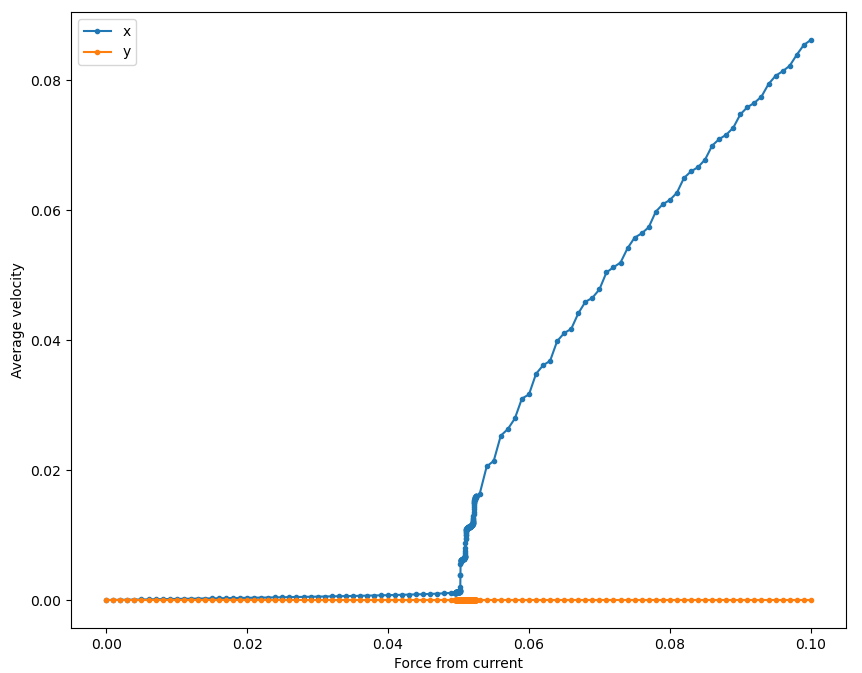
\includegraphics[width=.9\linewidth]{results/Figures/Width1_velocities_cutoff=9.png}
    \caption{Simulation of the channel using many stationary vortices.}
    \label{fig:big_vels_channel}
\end{subfigure}
\hfill
\begin{subfigure}[t]{.49\textwidth}
    \centering
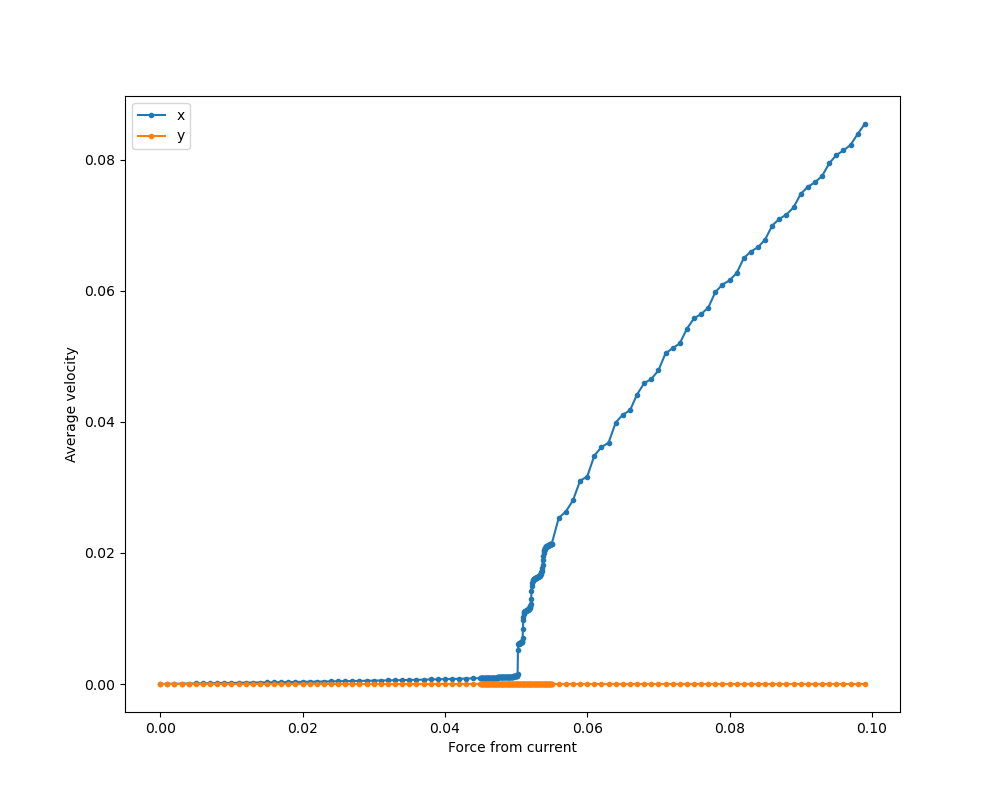
\includegraphics[width=.9\linewidth]{results/Figures/Width1_velocities_analytic_cutoff=9.png}
    \caption{Simulation of the channel using the form found from section~\ref{sec:analytic_chan}.}
    \label{fig:big_vels_analytic}
\end{subfigure}
\caption{Plots of the average vortex velocity for varying applied Lorentz forces.}
\label{fig:big_vels}
\end{figure}

Both of these plots show the expected form of the $F$-$v$ plot discussed in section~\ref{sec:critical_shear}, tending towards $F\propto v$ for higher applied forces with a cutoff critical shear below which $v=0$. The velocities due to forces near the critical shear are shown in figure~\ref{fig:fc_vels} again for both channel simulation methods. Both cases give a value for $F_c$ of around $0.0502$, an error of $0.4\%$ from the true value. Below this, $v$ remains just above zero due to the initial movement of the vortices up their potential wells before reaching a stationary equilibrium. Such a close value for the critical shear provides large confidence that the code is simulating the system correctly and to a high precision.

However, both methods show a stepping behaviour, most noticeable in figure~\ref{fig:fc_vels} due to the smaller steps in $F$ but still visible in figure~\ref{fig:big_vels}. The cause of this is unclear and may just be numerical error due to insufficient imaging grids, time steps or channel length. This would need to be investigated further should higher precision be required in such plots.

\begin{figure}[htb]
\centering
\begin{subfigure}[t]{.49\textwidth}
    \centering
    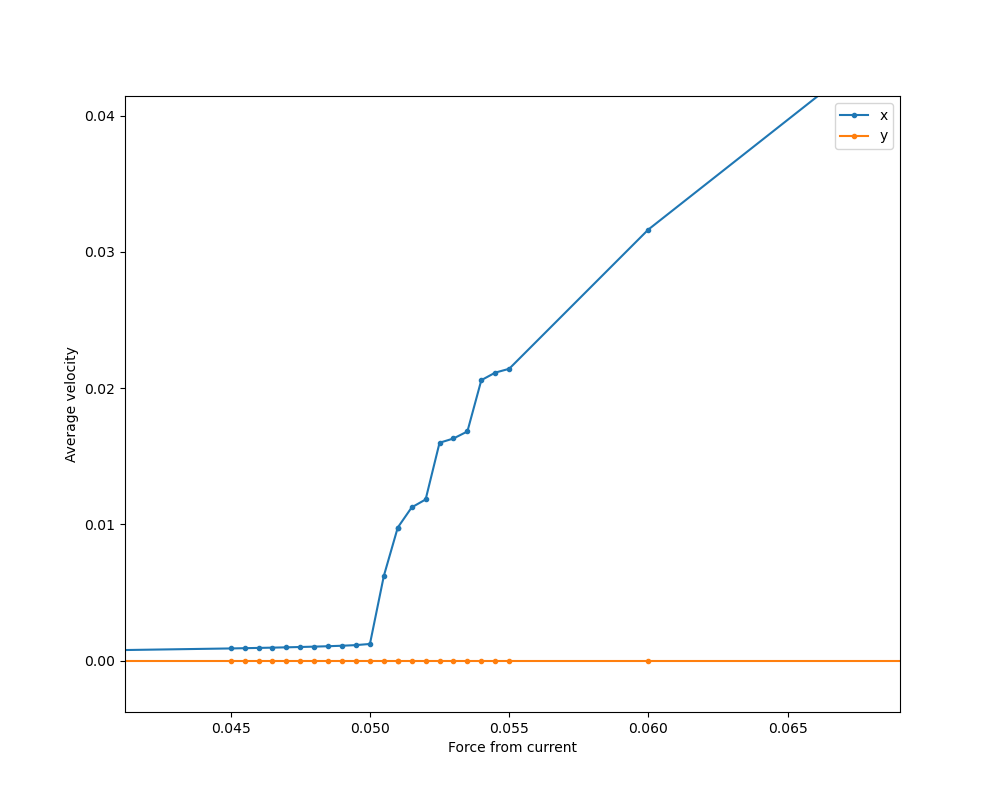
\includegraphics[width=.9\linewidth]{results/Figures/Width1_velocities_Fc.png}
    \caption{Simulation of the channel using pinned vortices.}
    \label{fig:fc_vels_channel}
\end{subfigure}
\hfill
\begin{subfigure}[t]{.49\textwidth}
    \centering
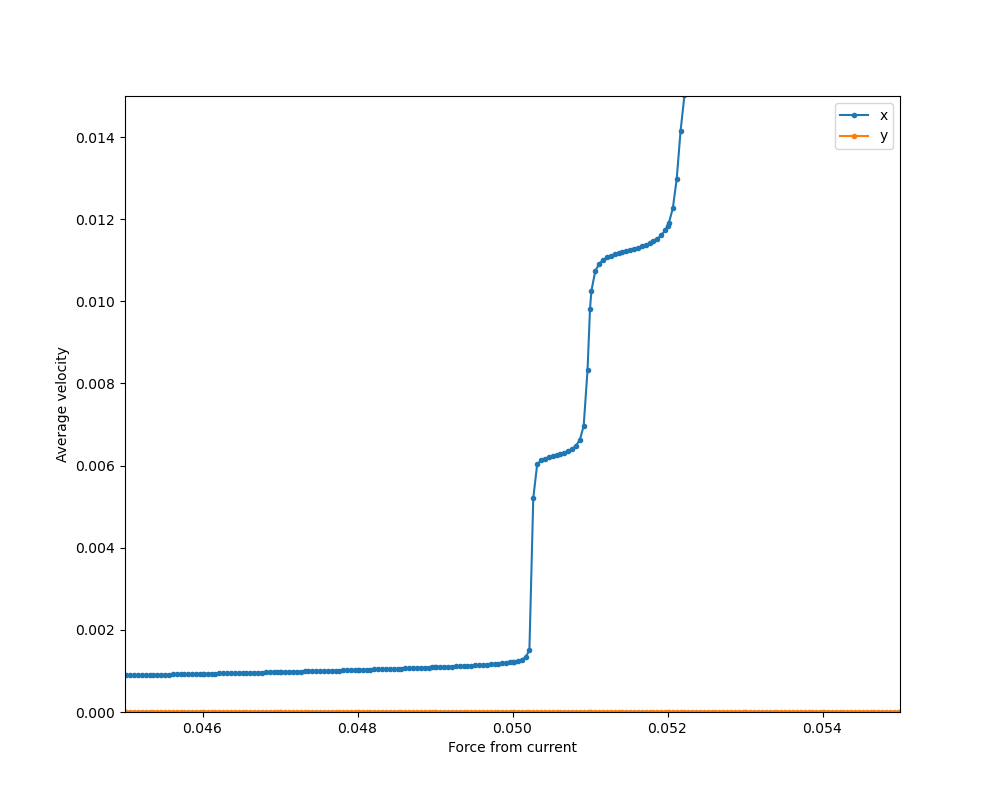
\includegraphics[width=.9\linewidth]{results/Figures/Width1_velocities_analytic_Fc.png}
    \caption{Simulation of the channel using the functional channel potential.}
    \label{fig:fc_vels_analytic}
\end{subfigure}
\caption{Plots of the average velocity near the critical shear $F_c$.}
\label{fig:fc_vels}
\end{figure}

\section{Next steps}
\subsection{Self-organised criticality}
In thermodynamics, a system near or at a phase transition is described as critical. Here small, local disturbances can affect the entire system rather than only the region near the disturbance with an exponentially decaying effect elsewhere. Achieving such behaviour in thermodynamic systems requires fine-tuning by external means so that the system may exist within the small critical region.

However, this kind of behaviour can also be seen outside of thermodynamics in systems such as a sand pile. When grains of sand are slowly added on to the top of a pile they generally will just add to the size of the slope. However, sometimes a single grain more causes an avalanche of sand to occur if the slope has reached a certain steepness. Such avalanches can range from very small if a limited slope has built up, to occasionally affecting up to the entire pile. What is notable here, is that such a system is naturally critical without any tuning of conditions as it brings itself to a state where large scale events can occur. This is called self-organised criticality (SOC), where a system is in a critical state for a wide range of parameters or initial states \cite{Tang1993SOCState, Jensen1998Self-organizedSystems}.

A key feature of SOC systems is the existence of power laws. Rather than the events being distributed by an exponential decay, they take the form $P(n)\sim n^{-\alpha}$, where in the case of the sand pile this could be the distribution of avalanches that contain $n$ grains. However, this distribution will reach a cut-off at which this power-law falls away based on a scale determined by - and due to - the finite size of the system. This form of distribution can be found in all self-organised critical systems to describe the magnitude or length of events within the system.

It is also important that SOC has a distinct separation of timescales between the lengths of events and their occurrences. Events must be suitably spaced that they are distinguishable from each other rather than blending into a more constant macroscopic effect. This leads to SOC often involving a gradually increasing force that at some point becomes great enough to create a sudden change in the system before building up again. The threshold at which an event occurs is unpredictable however, leading to the distribution of event sizes discussed previously \cite{Jensen1998Self-organizedSystems}.

\subsection{Vortex avalanches}
Previously, the pinning sites at which vortices are held have been assumed to exert a sufficiently large force on the vortices that a pinned vortex is immovable. However, such sites have a maximum pinning force, $F_p$, beyond which the vortex will escape the pinning site and flow elsewhere \cite{Poole2014Superconductivity}. In the case where an applied force $F$ is just below $F_p$, we see the phenomenon of flux creep. Here the vortices are almost able to escape their pinning sites and with a small random thermal kick, they can hop to the next pinning centre. This leads to the vortices slowly creeping along in the direction of the applied force.

However, in the case of low temperatures, such hopping very rarely occurs so vortices will remain pinned near the edge of the superconductor at which they are created. This build up pushes vortices away from the edge to balance the pinning force creating a gradient of vortex density in near equilibrium with the force from the pinning centres \cite{Tang1993SOCState}. This finally balanced, self-correcting equilibrium leads to a self-organised criticality state in which if one vortex is displaced, it will lead to an avalanche of displaced vortices as it leaves behind a free pinning site and forces others out of other sites.

These avalanches can have varying causes for them such as in \cite{Tang1993SOCState} where Tang discusses the case where events are caused by thermal fluctuations. However, there is no continuous addition of vortices to replace those that jump further into the superconductor meaning the vortex gradient is not maintained and the system tends to a uniform distribution of vortices. Field et al. \cite{Field1995SuperconductingAvalanches} instead kept a constant gradient by slowly raising the applied magnetic field. This causes new vortices to be added to the edge of the superconductor, much in the same way as in the sand pile model discussed previously. The addition of these vortices pushes the already existing vortices until an avalanche is triggered. After the avalanche, new vortices restore the vortex gradient again until another avalanche event occurs as we would expect in SOC. However, the slowly increasing applied field created an underlying flux flow which limited the resolution with which smaller avalanches could be detected.

\begin{figure}[htb]
    \centering
    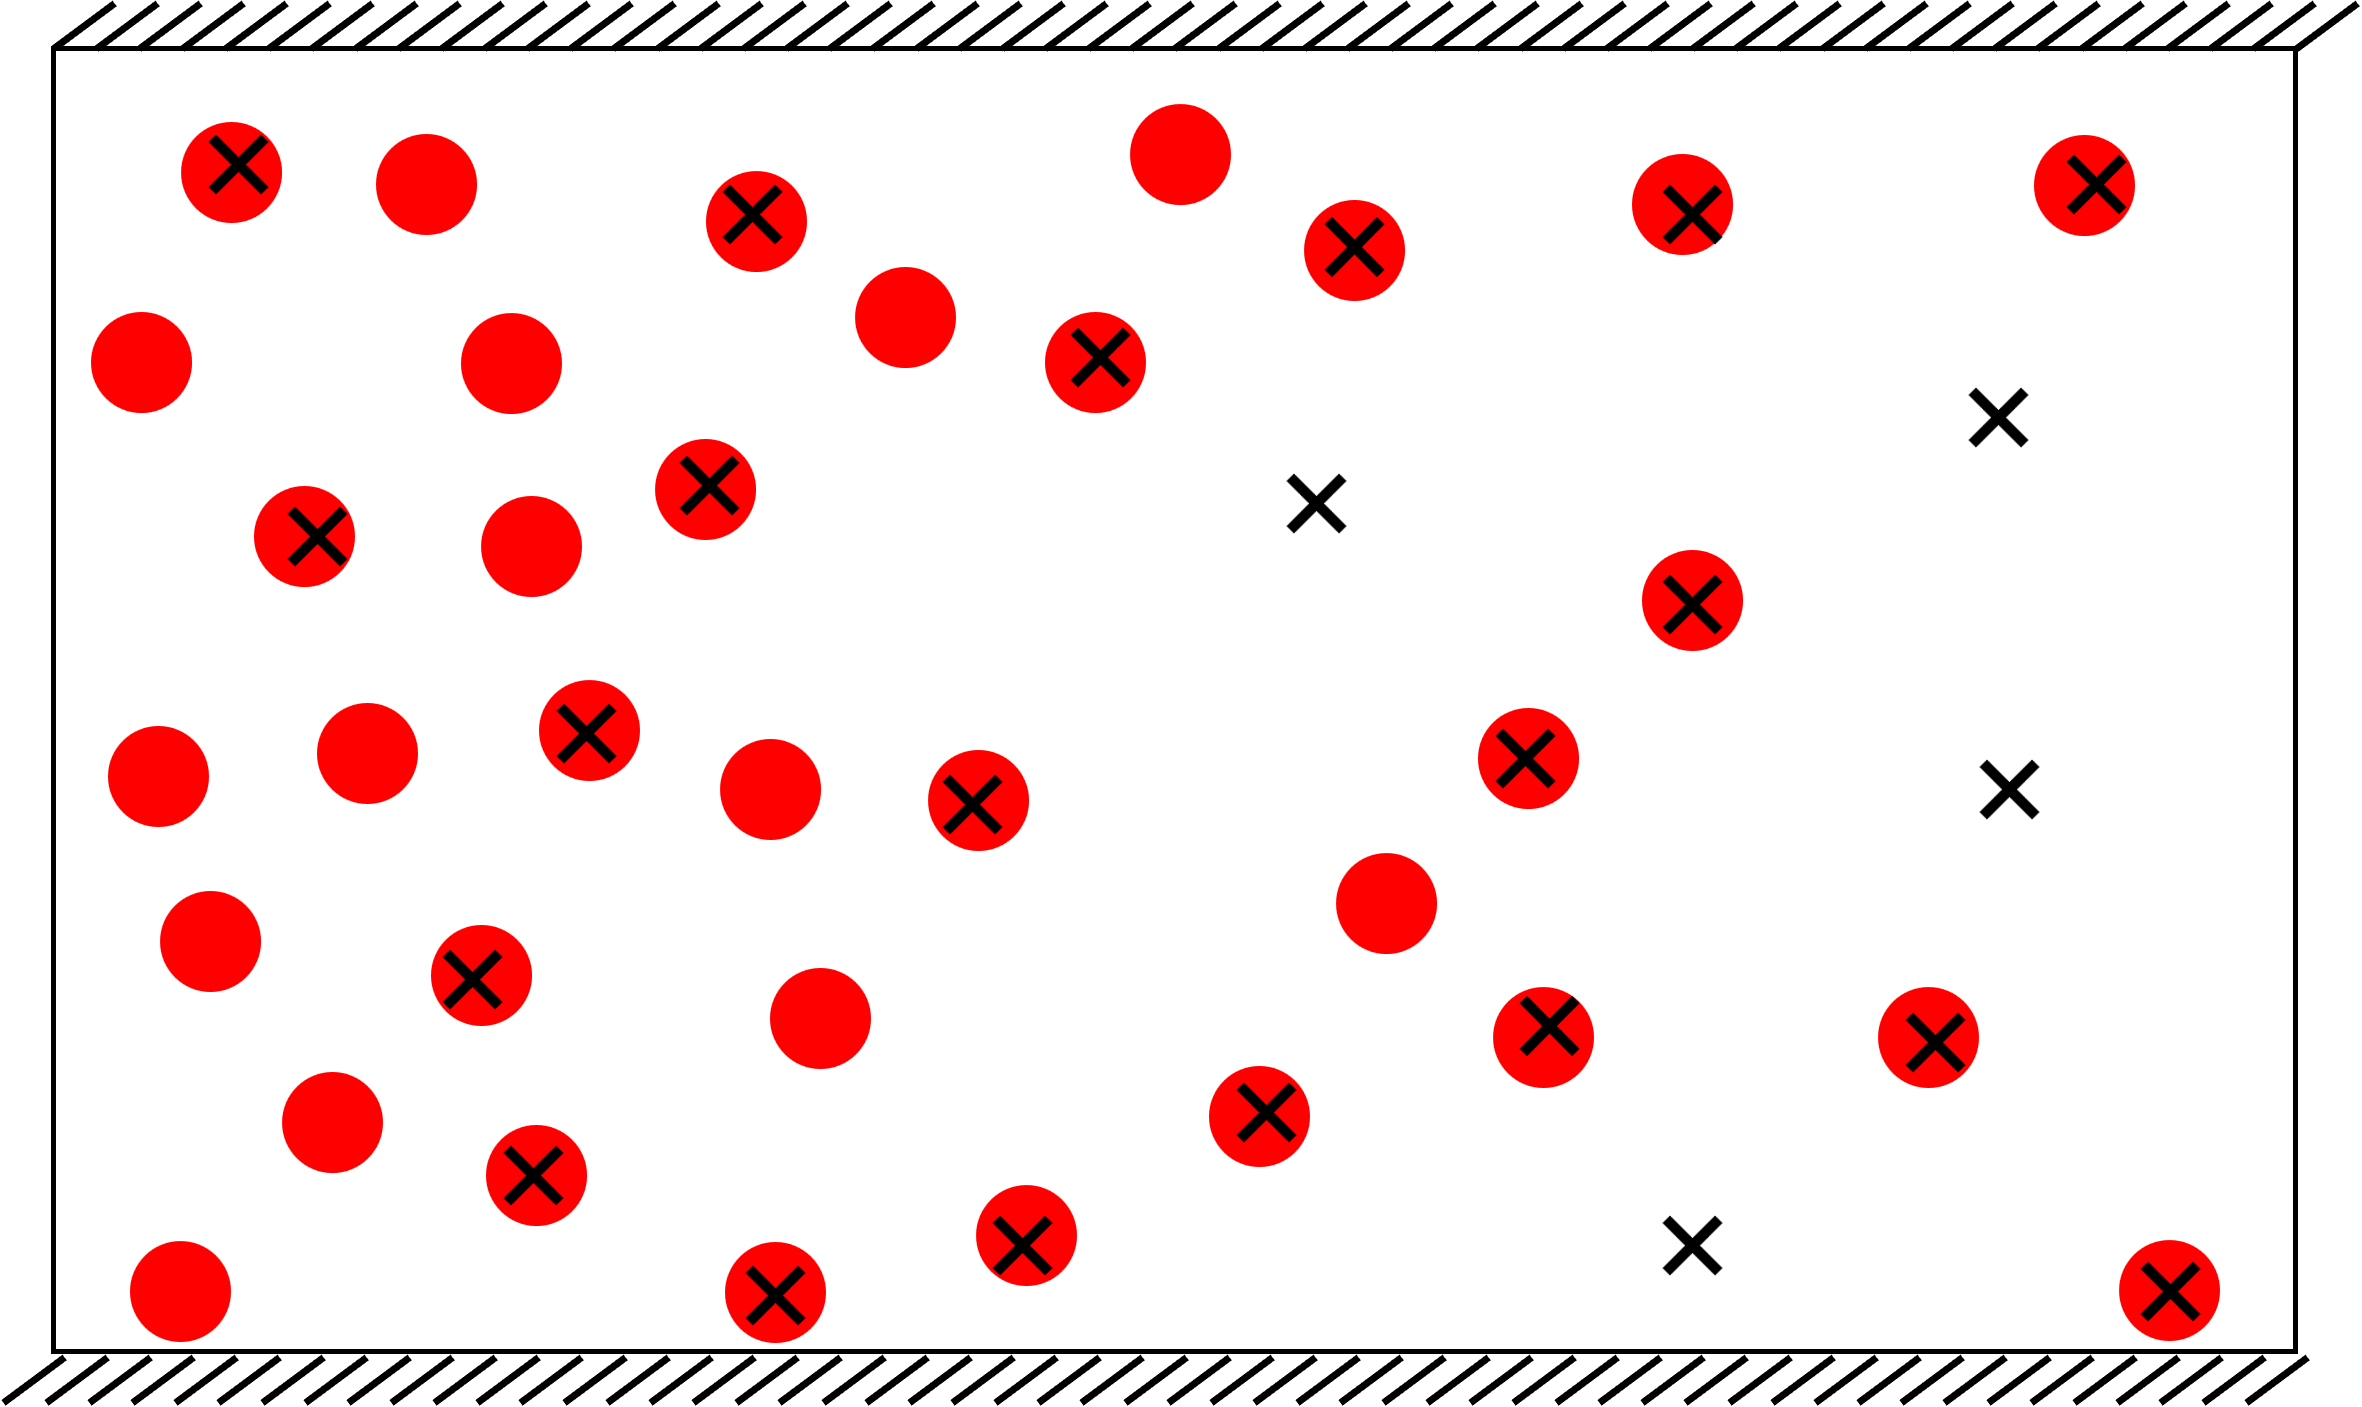
\includegraphics[width=0.8\linewidth]{Reports/ProjectProposal/Resources/avalanche_system.png}
    \caption{The vortex avalanche system. Crosses are randomly placed pinning sites, red dots are the location of the vortices. Vortices are slowly added to the left side of the system and removed if they pass the right-hand boundary.}
    \label{fig:avalanche_system}
\end{figure}
My project will be to investigate this system through an extension of the simulation code used previously. The avalanche system will be modelled as shown in figure~\ref{fig:avalanche_system} using periodic boundaries in the $y$ direction. A new vortex will be added to a random point on the left side and the system allowed to propagate. Any avalanches caused will be recorded and a new vortex added only when motion has ended. This ensures the separation of time scales discussed earlier as there is no danger of a second avalanche being started whilst another is still ongoing.

The crosses in figure~\ref{fig:avalanche_system} are randomly placed pinning sites, towards which vortices are attracted. I will investigate the effects of different potentials with which to model these sites. This could involve adjusting the size and strength of the potential as well as its functional form such as a Gaussian, step function or linear forms. These simulations will be used to produce phase plots such as those seen in \cite{Field1995SuperconductingAvalanches}. These give a probability distribution for differing sizes of avalanches from which the existence of power laws and scale invariance needed for SOC can be checked for.

\printbibliography

\end{document}
